\documentclass[11pt,a4paper]{article}

\usepackage{fontspec}
\usepackage{fontspec}
\usepackage[english, russian]{babel} % Russian — последний, значит основной

\setmainfont{cmunrm.otf}[
  BoldFont        = cmunbx.otf,
  ItalicFont      = cmunti.otf,
  BoldItalicFont  = cmunbi.otf
]


\usepackage[a4paper,margin=20mm]{geometry}
\usepackage{graphicx}
\usepackage{verbatim}
\usepackage{caption}
\usepackage{float}
\usepackage{hyperref}

\title{Результаты экспериментов \\
       \large Booth-умножитель с внешним recoder'ом}
\author{}
\date{\today}

\graphicspath{{../../py/figures/}}

\begin{document}


\section{Площадь}

\subsection{Сводная таблица}

\verbatiminput{../../syn/reports/summary_area.txt}

\section{Мощность}

\subsection{Сводная таблица}

\verbatiminput{../../pwr/reports/summary_power.txt}

\subsection{Сравнение конфигураций (gauss\_slow)}

\begin{figure}[H]
    \centering
    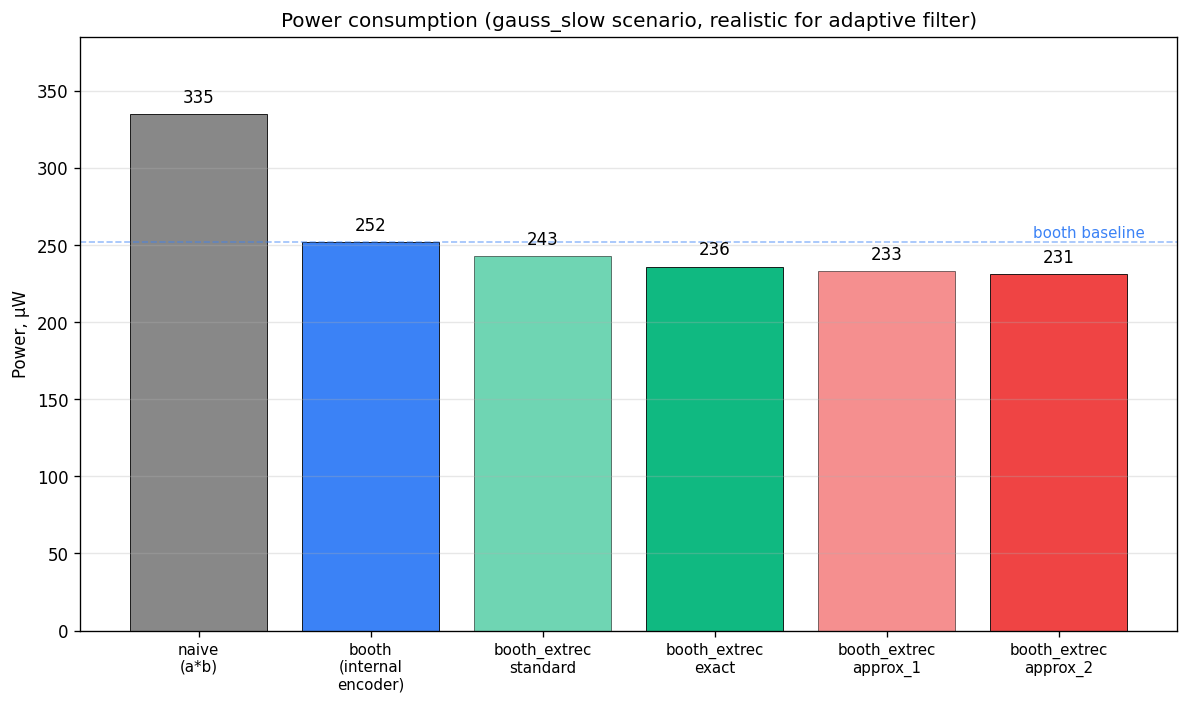
\includegraphics[width=0.9\textwidth]{power_dut_comparison_gauss_slow.png}
    \caption{Мощность всех конфигураций умножителя в сценарии gauss\_slow.}
\end{figure}

\subsection{Мощность booth\_extrec по уровню recoding}

\begin{figure}[H]
    \centering
    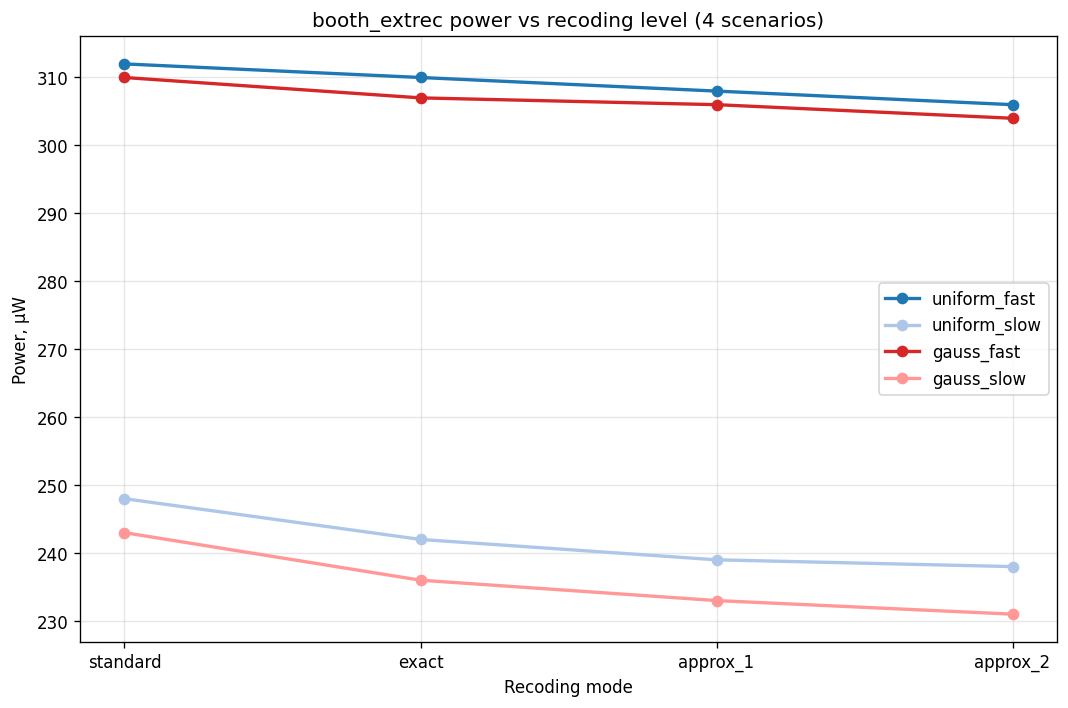
\includegraphics[width=0.9\textwidth]{power_extrec_vs_recoding_mode.png}
    \caption{Мощность booth\_extrec в зависимости от режима recoding для четырёх сценариев стимулов.}
\end{figure}

\section{Точность}

\subsection{Сводная таблица}

\verbatiminput{../../py/reports/summary_accuracy.txt}

\subsection{Метрики точности по уровню recoding}

\begin{figure}[H]
    \centering
    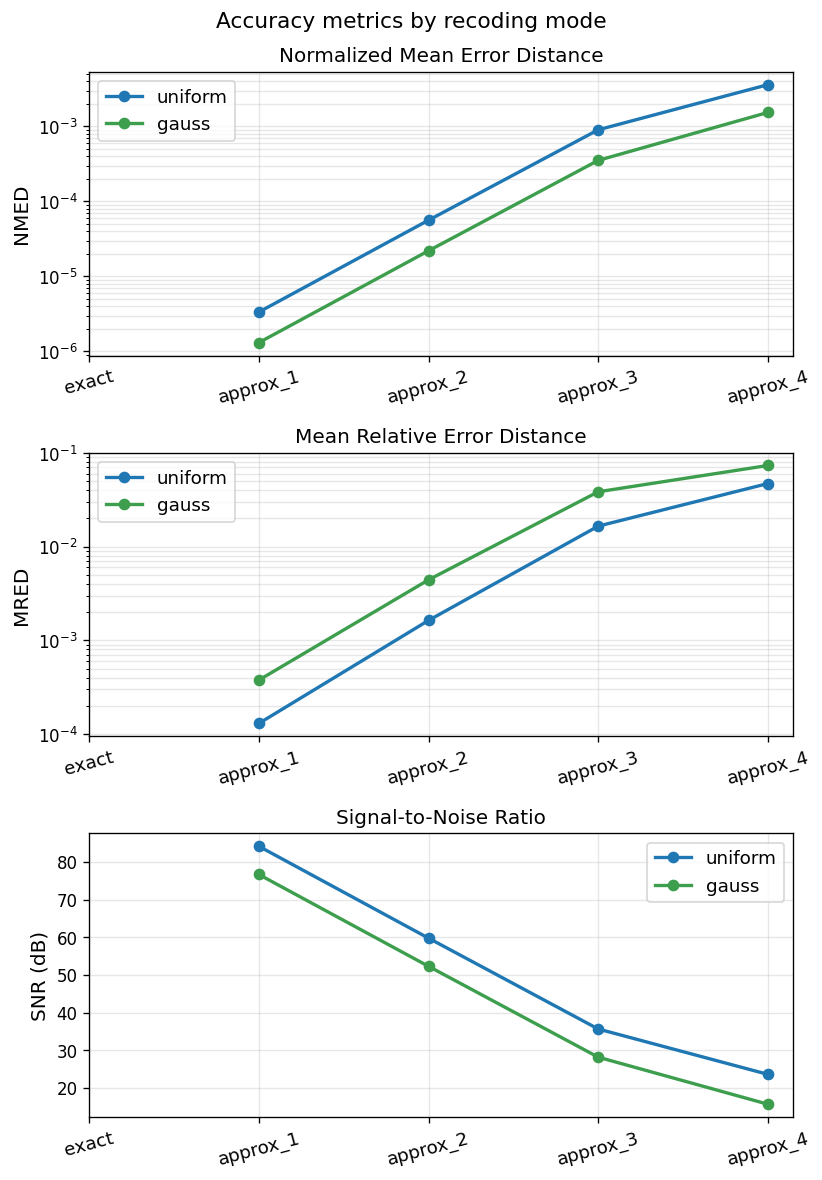
\includegraphics[width=\textwidth]{accuracy_nmed_mred_snr.png}
    \caption{NMED, MRED и SNR в зависимости от режима recoding для uniform и gauss распределений.}
\end{figure}

\section{Статистика паттернов}

\subsection{Среднее число нулевых строк PP-матрицы}

\begin{figure}[H]
    \centering
    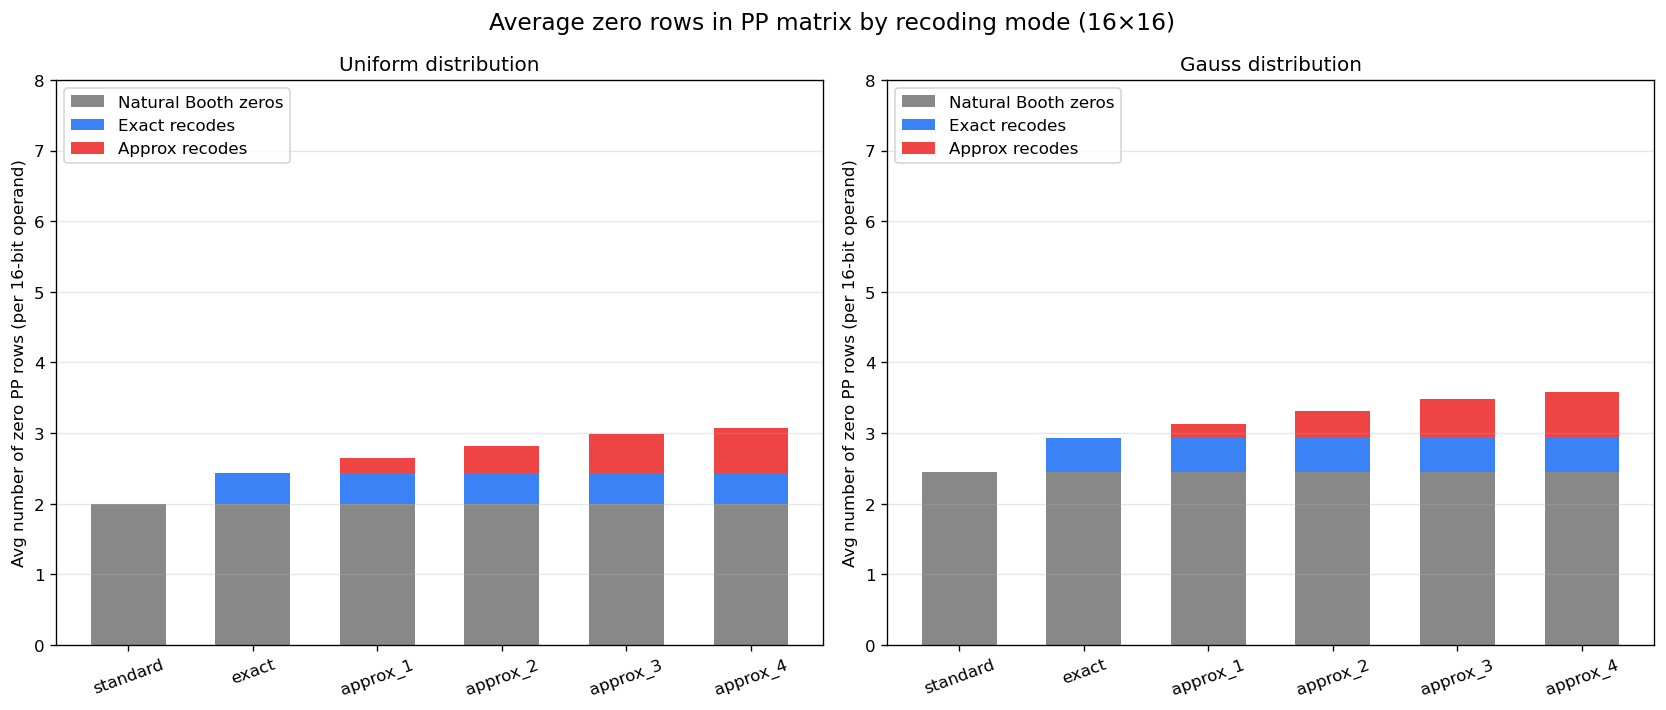
\includegraphics[width=\textwidth]{patterns_zero_rows_by_mode.png}
    \caption{Среднее число нулевых строк partial product матрицы (natural + exact recodes + approx recodes) по режимам recoding для двух распределений.}
\end{figure}

\end{document}